\documentclass[a4paper, 11pt,oneside]{article}
\usepackage[
  top=1.5cm,
  bottom=1cm,
  left=2cm,
  right=1.5cm,
  headheight=25.22153pt, % as per the warning by fancyhdr
  includehead,includefoot,
  heightrounded, % to avoid spurious underfull messages
]{geometry} 

\usepackage[T1]{fontenc}
\usepackage{microtype}
\usepackage{fancyhdr}
\usepackage{fancyvrb}
\usepackage{lipsum}
\usepackage{url}
\usepackage{listings}
\usepackage{lastpage}
\usepackage{enumitem}
\usepackage{datetime}
\usepackage{amsthm}
\usepackage{graphicx}
\usepackage{hyperref}
\usepackage{minted}
\usepackage{float}

\settimeformat{hhmmsstime}
\yyyymmdddate

\pagestyle{fancy}
\fancyhf{} % clear all fields

\pagestyle{fancy}
\lhead{CMSC 132: Computer Architecture \\ First Semester 2020-2021}
\rhead{Institute of Computer Science \\ University of the 
Philippines Los Banos}
\rfoot{$\copyright$JACHermocilla (CC NC-BY-SA 4.0)}
%\cfoot{Enjoy!:)}
\cfoot{\thepage\ of \pageref{LastPage}}
\lfoot{Revision: \today\ \currenttime}
%\rfoot{https://jachermocilla.org/teaching/125}
\renewcommand{\headrulewidth}{0.4pt}
\renewcommand{\footrulewidth}{0.4pt}

\begin{document}

\begin{center}
	{\LARGE \textbf{Instruction Set Architecture Design and Implementation}}
\end{center}

\section*{Learning Outcomes}
   At the end of this lab, you should be able to:
   \begin{enumerate}[itemsep=0pt,parsep=0pt]
   	   \item design and implement a simple ISA;
       \item write a simple assembler
   \end{enumerate}   
\tableofcontents

\section{Resources}
\begin{itemize}
	\item Video: \href{https://youtu.be/CzyXb_T-xgU}{https://youtu.be/CzyXb\_T-xgU}.
	\item Source Codes: \href{https://git.io/JU3al}{https://git.io/JU3al}
	\item Online VHDL Tool: \href{https://www.edaplayground.com/home}
	{https://www.edaplayground.com/home}
\end{itemize}	

\section{Discussion}
The \textbf{processor(CPU)} is composed of the \textbf{datapath} and 
\textbf{control}. In the previous labs, you learned that combinational and 
sequential circuit elements are used as building blocks to create the 
functional components of the datapath and control. Examples of these functional 
elements include the \textbf{ALU, Register File, Program Counter, and Memory}. 
You also learned that a \textbf{clock} drives the execution and control is 
implemented using a \textbf{finite state machine} for 
\textbf{fetch-decode-execute cycle}. One question that we can answer next is: 
\textit{How do we program the CPU?}


\subsection{Instruction Set Architecture}
Instruction Set Architecture (ISA) is an \textbf{abstraction} between the 
hardware and the lowest-level software. It includes anything programmers need 
to know to make a binary machine language program work correctly.


allows computer designers to talk about functions indepedently from the 
hardware that performs them.


%%\begin{figure}[H]
%%	\begin{center}
%%	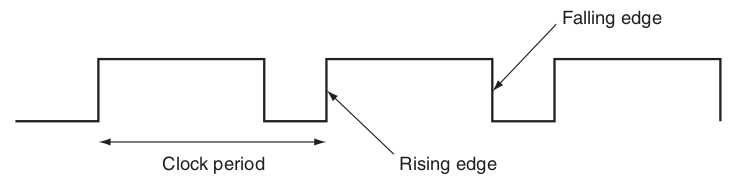
\includegraphics[width=4in]{clock0.png}
%%	\caption{A clock signal showin the clock period, falling edge, and rising 
%%edge.}
%%	\label{fig:clock0} 
%%	\end{center}
%%\end{figure}


\begin{minted}[frame=single,framesep=10pt]{vhdl}
LIBRARY ieee;
USE ieee.std_logic_1164.all;
ENTITY clocker_tb IS
END clocker_tb;
ARCHITECTURE behavior OF clocker_tb IS
   --100Mhz
   CONSTANT frequency: integer := 100e6; 
   CONSTANT period : time := 1000 ms / frequency;
   SIGNAL clk : std_logic := '0';
BEGIN 
   clk <= not clk after period / 2;
   -- do some stuff here using clk as input
END ARCHITECTURE;
\end{minted}

\section{Summary}
In this lab, you learned some of the sequential elements that are useful in the 
design of a processor as well as the importance of clocks. We also showed the
design and implementation of a simple traffic light system using finite state 
machines since a simple truth table is not enough to characterize a sequential 
system. 

You should now be able to tell whether a functional component of a datapath and 
control is composed of a combinational or sequential element.

\section{Learning Activities}
Download the source codes for this lab then try experimenting by adding more 
test cases in the testbenches. Submit a PDF document that shows screenshots of 
your modifications and runs. 

\section{Self-Assessment Questions}
\begin{enumerate}
\item What is the main purpose of clocks in sequential circuits?
\item What is the difference between a clocked latch and a flip-flop?
\item Why can't a multiplexer be used in RAM?
\item Why is SRAM more expensive than DRAM?
\item If my CPU is clocked at 800 MHz, what is the period?
\end{enumerate}


\section{Deliverable}
Your final deliverable for this lab is implement the RAM in Figure 
 \ref{fig:sram3}. Submit the VHDL code including a testbench as well as images 
of the waveforms. NOTE: Enable lines should be connected to the output of the 
decoder and the rightmost Din in the figure should be Din[0].

\section{Further Reading}
\begin{itemize}
\item 
\href{https://www.doulos.com/knowhow/vhdl/simple-ram-model/}
{https://www.doulos.com/knowhow/vhdl/simple-ram-model/}
\end{itemize}


%\begin{thebibliography}{9}
%\end{thebibliography}

\bibliographystyle{unsrt}
\bibliography{toma}
\nocite{*}

\end{document}